\documentclass[10pt]{article}
\usepackage[top=1in, bottom=1.2in]{geometry}
\linespread{1} % line spacing
\geometry{letterpaper}
\usepackage{tabularx}
\usepackage[parfill]{parskip} % begin paragraphs with an empty line rather than an indent
\usepackage[ocgcolorlinks]{hyperref} %ocg coverts links to black when you print -- downside of unbreakable lines



% New command \CustomLabel{labelname} creates a hypertarget and label for referencing
\makeatletter
 \newcommand{\CustomLabel}[1]{\Hy@raisedlink{\hypertarget{#1}{}}\label{#1}}
\makeatother

% Graph Stuff
\usepackage{tikz}
\usetikzlibrary{trees} % this is to allow the fork right path
\usetikzlibrary{calc} % for hyperlinking nodes

% Styling for Graphs
\tikzset{
    basic/.style  = {thin, draw, text width=5em, font=\sffamily, rectangle, minimum size=2em, align=center},
    root/.style   = {basic},
    edge from parent fork down,
        level 2/.style = {basic, grow=down, edge from parent path={(\tikzparentnode.south) |- (\tikzchildnode.west)}},
        level 3/.style = {basic, xshift=1ex,anchor=west},
            subA/.style={level distance=6ex},
            subB/.style={level distance=12ex},
            subC/.style={level distance=18ex},
    hyperlink node/.style={
      postaction={
        path picture={
          \path let
          \p1 = (path picture bounding box.south west),
          \p2 = (path picture bounding box.north east),
          \p3 = (\x2-\x1,\y2-\y1)
          in
          (path picture bounding box.center)
          node[inner sep=0pt,anchor=center,outer sep=0pt]
          {\hyperlink{#1}{\phantom{\rule{\x3}{\y3}}}};
        }
      },
    }
}

\title{\bf Checkers Design Document}
\author{me 3}
\date{}

\begin{document} %%%%%%%%%%%%%%%%%%%%%%%%%%%%%%%%%%%%%%%%%%%%%%%%%%%%%%%%%%%%%%%%%%%%%%%%%%
\maketitle

\tableofcontents

\section{Introduction}
    This document contains decomposition (MG and MIS), uses relationship, and traceability.
    
\section{Module Guide}
Modules are stuff.

\subsection{Hardware Hiding Module}
\iffalse
    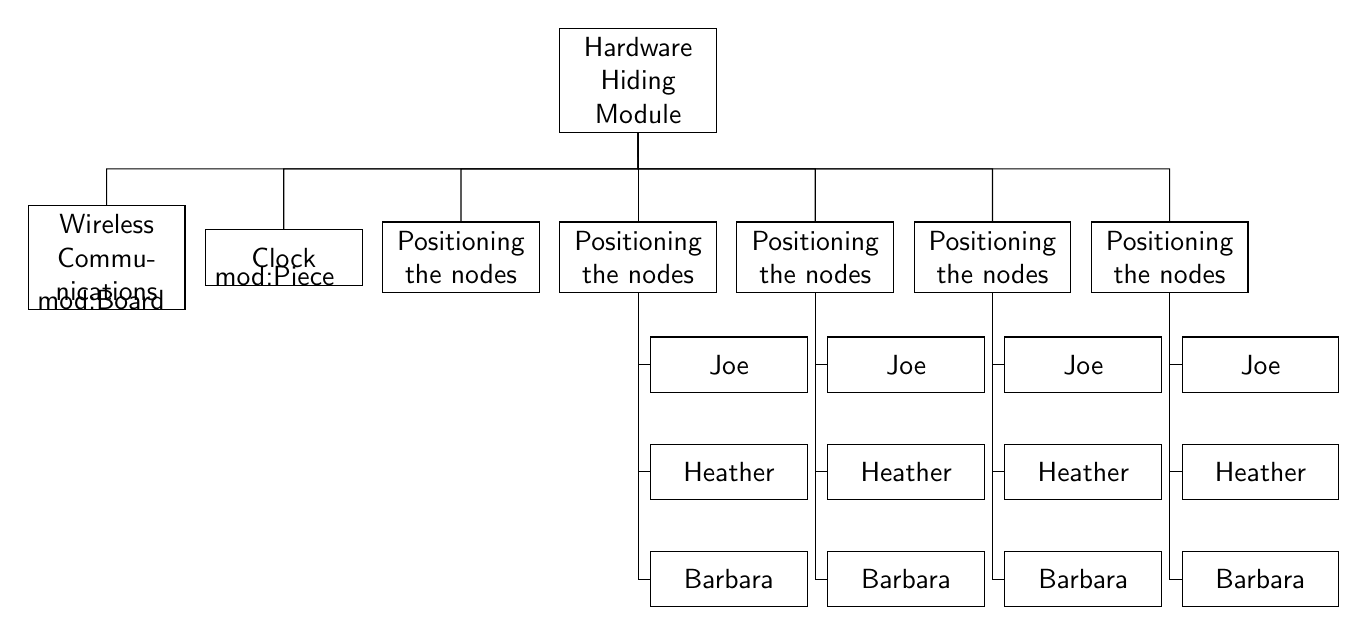
\begin{tikzpicture}[scale=1.5, align=center]
        \node[root] {Hardware Hiding Module}
        child {node[level 2, hyperlink node=mod:Board]{Wireless Communications}}
        child {node[level 2, hyperlink node=mod:Piece]{Clock}}
        child {node[level 2]{Positioning the nodes}}
        child {node[level 2]{Positioning the nodes}
            child[subA] {node[level 3]{Joe}}
            child[subB] {node[level 3]{Heather}}
            child[subC] {node[level 3]{Barbara}}}
        child {node[level 2]{Positioning the nodes}
            child[subA] {node[level 3]{Joe}}
            child[subB] {node[level 3]{Heather}}
            child[subC] {node[level 3]{Barbara}}}
        child {node[level 2]{Positioning the nodes}
            child[subA] {node[level 3]{Joe}}
            child[subB] {node[level 3]{Heather}}
            child[subC] {node[level 3]{Barbara}}}
        child {node[level 2]{Positioning the nodes}
            child[subA] {node[level 3]{Joe}}
            child[subB] {node[level 3]{Heather}}
            child[subC] {node[level 3]{Barbara}}}
        ;
    \end{tikzpicture}
\fi
    
\subsection{Behaviour Hiding Module}

\subsection{Software Decision Hiding Module}

    \subsubsection{Piece Module}\CustomLabel{mod:Piece}
        \begin{tabularx}{\linewidth}{ >{\bfseries}r X }
            Type            & Software Module \\
            Secret          & This module hides and separates specific piece information. \\
            Responsibilites & This will hold the necessary components to describe what a game piece will contain, which will be seperate from the game board. \\
            Uses            & None \\
            Design          & \ref{mis:Piece} \\
        \end{tabularx}
                
                
    \subsubsection{Board Module}\CustomLabel{mod:Board}
        \begin{tabularx}{\linewidth}{ >{\bfseries}r X }
            Type            & Software Module \\
            Secret          & This module serves to hide the secret of how the board is defined internally. \\
            Responsibilites & This module is responsible for holding the necessary components and attributes to setup the board and describe piece locations. \\
            Uses            & \ref{mod:Piece} \\
            Design          & \ref{mis:Board} \\
        \end{tabularx}
        
        
\newpage
%%%%%%%%%%%%%%%%%%%%%%%%%%%%%%%%%%%%%%%%%%%%%%%%%%%%%%%%%%%%%%%%%%%%%%%%%%%%%%%%%%%%%%%%%%%%%%%%%%%%%%



\section{Module Interface Specification}


        
        
    \subsection{Piece Module}\CustomLabel{mis:Piece}
    \subsubsection{Interface}
        \begin{tabularx}{\linewidth}{@{} >{\bfseries}r Xp{5cm} }
            Types           & \begin{tabular}[t]{@{} l p{8cm}} 
                                     & \\
                                    typeState & enumerate if the piece is normal or king \\
                                    player & enumerate if piece owned by Black or White \\
                              \end{tabular} \\
                              
            Constants       & \begin{tabular}[t]{@{} l p{8cm}} 
                                     & \\
                                    None & \\
                              \end{tabular} \\

            Access Programs & \begin{tabular}[t]{@{} l p{8cm}}
                                     & \\
                                    getType() & Retrieves the piece's current type. \\
                                    setType(newType : typeState) & Changes the piece's type. \\ 
                                    getOwner() & Says who owns the piece. \\
                              \end{tabular}
        \end{tabularx}
        
    \subsubsection{Implementation}
        \begin{tabularx}{\linewidth}{ >{\bfseries}r Xp{5cm} }
            Variables       & \begin{tabular}[t]{@{} l p{8cm}} 
                                     & \\
                                    pieceType : typeState & holds current piece type \\
                                    owner : player & holds information of the piece's owner \\
                              \end{tabular} \\

            Access Programs & \begin{tabular}[t]{@{} l l p{8cm}} 
                                     & \\
                                    \bf{getType()} & \\
                                    Inputs &  None \\
                                    Outputs & pieceType \\
                                    Updates & None \\ 
                                     & \\
                                    \bf{setType(newType : typeState)} & \\
                                    Inputs & newType \\
                                    Outputs & None \\
                                    Updates & pieceType \\ 
                                     & \\
                                    \bf{getOwner()} & \\
                                    Inputs & None \\
                                    Outputs & owner \\
                                    Updates & None \\ 
                              \end{tabular} \\
                              
        \end{tabularx}
        
        
        
        
        
        
            \subsection{Board Module}\CustomLabel{mis:Board}
    \subsubsection{Interface}
        \begin{tabularx}{\linewidth}{@{} >{\bfseries}r Xp{5cm} }
            Types           & \begin{tabular}[t]{@{} l p{8cm}} 
                                     & \\
                                    None & \\
                              \end{tabular} \\
                              
            Constants       & \begin{tabular}[t]{@{} l p{8cm}} 
                                     & \\
                                    None & \\
                              \end{tabular} \\

            Access Programs & \begin{tabular}[t]{@{} p{4cm} p{8cm}}
                                     & \\
                                    clear() & Removes all pieces from the board. \\
                                     & \\
                                    placePiece(col : int, row : int, piece : Piece) & Places the piece on the board while checking if the placement is legal (in terms of checkers). \\
                                     & \\
                                    movePiece(fromCol : int, fromRow : int, toCol : int, toRow : int) & Moves the piece from starting to end positions while checking if the movement is valid (in terms of checkers). \\
                                     & \\
                                    getPiece(col : int, row : int) & This method is used to determine if a piece exists on a square of the board. If the piece does exist, we pass it along to the caller. \\ 
                             \end{tabular}
        \end{tabularx}
        
    \subsubsection{Implementation}
        \begin{tabularx}{\linewidth}{ >{\bfseries}r Xp{5cm} }
            Types           & \begin{tabular}[t]{@{} l p{8cm}} 
                                 & \\
                                None & \\
                            \end{tabular} \\
                            
            Constants       & \begin{tabular}[t]{@{} l p{8cm}} 
                                 & \\
                                None & \\
                            \end{tabular} \\
                              
            Variables       & \begin{tabular}[t]{@{} l p{8cm}} 
                                     & \\
                                    pieceArray[] & The board will be implemented as an array. \\
                              \end{tabular} \\

            Access Programs & \begin{tabular}[t]{@{} p{6cm} p{8cm}} 
                                     & \\
                                    \bf{clear()} & \\
                                    Inputs & None \\
                                    Outputs & pieceArray[] \\
                                    Updates & None \\ 
                                     & \\
                                    \bf{placePiece(col : int, row : int, piece : Piece)} & \\
                                    Inputs &  col, row, piece \\
                                    Outputs & pieceArray[] \\
                                    Updates & None \\ 
                                     & \\
                                    \bf{movePiece(fromCol : int, fromRow : int, toCol : int, toRow : int)} & \\
                                    Inputs & None \\
                                    Outputs & None \\
                                    Updates & None \\
                                     & \\
                                    \bf{getPiece(col : int, row : int)} & \\
                                    Inputs & col, row \\
                                    Outputs & piece \\
                                    Updates & None \\                                     
                              \end{tabular} \\
                              
        \end{tabularx}
        

        
\end{document}












